	\subsection{UC 7 - Ente - Gestione utenti}

		\begin{figure}[H]
			\centering
			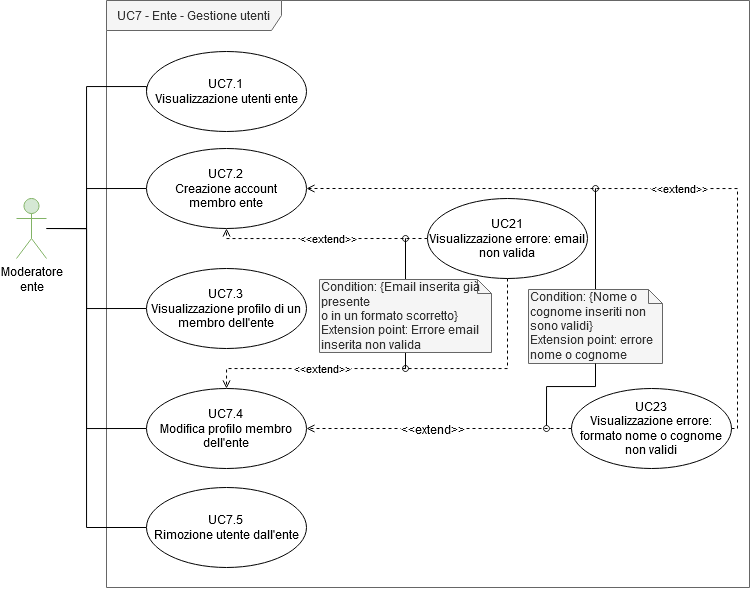
\includegraphics[scale=0.60]{res/images/uc7}
			\caption{Diagramma che riassume la gestione utenti appartenenti a un ente nella web app.}
		\end{figure}

		\begin{itemize}
			\item \textbf{attori primari:} moderatore ente;
			\item \textbf{descrizione:} l'utente può gestire gli utenti del proprio ente, eseguendo modifiche e cancellazioni di account esistenti o aggiunte di nuovi account;
			\item \textbf{precondizione:} l'utente è autenticato e naviga nella gestione utenti per l'ente associato;
			\item \textbf{postcondizione:} l'utente ha visualizzato o gestito gli utenti appartenenti al proprio ente;
			\item \textbf{scenario principale:}
			\begin{enumerate}
				\item{l'utente visualizza o gestisce gli utenti appartenenti al proprio ente.}
			\end{enumerate}
		\end{itemize}

			\subsubsection{UC 7.1 - Visualizzazione utenti ente}
			\begin{itemize}
				\item \textbf{attori primari:} moderatore ente;
				\item \textbf{descrizione:} l'utente può visualizzare una lista con nome, cognome e mail degli utenti del proprio ente;
				\item \textbf{precondizione:} l'utente naviga nella gestione utenti per l'ente associato;
				\item \textbf{postcondizione:} l'utente ha visualizzato la lista degli utenti appartenenti al proprio ente;
				\item \textbf{scenario principale:}
				\begin{enumerate}
					\item{l'utente visualizza la lista degli utenti appartenenti al proprio ente.}
				\end{enumerate}
			\end{itemize}

			\subsubsection{UC 7.2 - Creazione account membro ente}
			\begin{itemize}
				\item \textbf{attori primari:} moderatore ente;
				\item \textbf{descrizione:} l'utente può creare un nuovo membro per il proprio ente;
				\item \textbf{precondizione:} l'utente naviga nella gestione utenti per l'ente associato;
				\item \textbf{postcondizione:} l'utente ha creato un nuovo account associato al proprio ente;
				\item \textbf{scenario principale:}
				\begin{enumerate}
					\item{l'utente deve compilare dei campi obbligatori per aggiungere un nuovo utente;}
					\item{l'utente compila il campo email (UC 7.2.1);}
					\item{l'utente compila il campo nome (UC 7.2.2);}
					\item{l'utente compila il campo cognome (UC 7.2.3);}
					\item{l'utente ha aggiunto un nuovo utente appartenente al proprio ente;}
				\end{enumerate}
				\item \textbf{estensioni:}
				\begin{itemize}
					\item l'utente inserisce un email non valida (UC 21);
					\item l'utente inserisce un nome o cognome non validi (UC 23).
				\end{itemize}
			\end{itemize}

			\paragraph{UC 7.2.1 - Inserimento email}
			\begin{itemize}
				\item \textbf{attori primari:} moderatore ente;
				\item \textbf{descrizione:} l'utente sta aggiungendo un nuovo utente e gli viene richiesto di compilare il campo obbligatorio per la email;
				\item \textbf{precondizione:} l'utente sta compilando i campi richiesti per l'aggiunta di un nuovo utente;
				\item \textbf{postcondizione:} l'utente ha compilato il campo richiesto per la creazione di un nuovo membro;
				\item \textbf{scenario principale:}
				\begin{enumerate}
					\item{l'utente ha compilato la email per il nuovo utente.}
				\end{enumerate}
			\end{itemize}

			\paragraph{UC 7.2.2 - Inserimento nome}
			\begin{itemize}
				\item \textbf{attori primari:} moderatore ente;
				\item \textbf{descrizione:} l'utente sta aggiungendo un nuovo utente e gli viene richiesto di compilare il campo obbligatorio per il nome;
				\item \textbf{precondizione:} l'utente sta compilando i campi richiesti per l'aggiunta di un nuovo utente;
				\item \textbf{postcondizione:} l'utente ha compilato il campo richiesto per la creazione di un nuovo membro;
				\item \textbf{scenario principale:}
				\begin{enumerate}
					\item{l'utente ha compilato il nome per il nuovo utente.}
				\end{enumerate}
			\end{itemize}

			\paragraph{UC 7.2.3 - Inserimento cognome}
			\begin{itemize}
				\item \textbf{attori primari:} moderatore ente;
				\item \textbf{descrizione:} l'utente sta aggiungendo un nuovo utente e gli viene richiesto di compilare il campo obbligatorio per il cognome;
				\item \textbf{precondizione:} l'utente sta compilando i campi richiesti per l'aggiunta di un nuovo utente;
				\item \textbf{postcondizione:} l'utente ha compilato il campo richiesto per la creazione di un nuovo membro;
				\item \textbf{scenario principale:}
				\begin{enumerate}
					\item{l'utente ha compilato il cognome per il nuovo utente.}
				\end{enumerate}
			\end{itemize}

			\subsubsection{UC 7.3 - Visualizzazione profilo di un membro dell'ente}
			\begin{itemize}
				\item \textbf{attori primari:} moderatore ente;
				\item \textbf{descrizione:} l'utente può visualizzare nome, cognome, mail, username Telegram (se presente) e l'opzione di autenticazione a due fattori (attiva o meno) dell'utente selezionato dalla lista degli utenti del proprio ente;
				\item \textbf{precondizione:} l'utente naviga nella gestione utenti per l'ente associato e visualizza i propri membri;
				\item \textbf{postcondizione:} l'utente ha visualizzato i dati dell'utente selezionato appartenente al proprio ente;
				\item \textbf{scenario principale:}
				\begin{enumerate}
					\item{l'utente seleziona un utente dalla lista degli utenti del proprio ente;}
					\item{l'utente visualizza i dati dell'utente selezionato.}
				\end{enumerate}
			\end{itemize}


			\subsubsection{UC 7.4 - Modifica account membro ente}
			\begin{itemize}
				\item \textbf{attori primari:} moderatore ente;
				\item \textbf{descrizione:} l'utente può modificare un membro del proprio ente;
				\item \textbf{precondizione:} l'utente naviga nella gestione utenti per l'ente associato;
				\item \textbf{postcondizione:} l'utente ha modificato un nuovo account associato al proprio ente;
				\item \textbf{scenario principale:}
				\begin{enumerate}
					\item{l'utente deve compilare dei campi obbligatori per modificare un utente;}
					\item{l'utente compila il campo email (UC 7.4.1);}
					\item{l'utente compila il campo nome (UC 7.4.2);}
					\item{l'utente compila il campo cognome (UC 7.4.3);}
					\item{l'utente ha modificato un utente appartenente al proprio ente;}
				\end{enumerate}
				\item \textbf{estensioni:}
				\begin{itemize}
					\item l'utente inserisce un email non valida (UC 21);
					\item l'utente inserisce un nome o cognome non validi (UC 23).
				\end{itemize}
			\end{itemize}

			\paragraph{UC 7.4.1 - Modifica campo email}
			\begin{itemize}
				\item \textbf{attori primari:} moderatore ente;
				\item \textbf{descrizione:} l'utente sta modificando un utente e gli viene richiesto di compilare il campo obbligatorio per la email;
				\item \textbf{precondizione:} l'utente sta compilando i campi richiesti per la modifica di un utente;
				\item \textbf{postcondizione:} l'utente ha compilato il campo richiesto per la modifica di un membro;
				\item \textbf{scenario principale:}
				\begin{enumerate}
					\item{l'utente ha compilato la email dell'utente.}
				\end{enumerate}
			\end{itemize}

			\paragraph{UC 7.4.2 - Modifica campo nome}
			\begin{itemize}
				\item \textbf{attori primari:} moderatore ente;
				\item \textbf{descrizione:} l'utente sta modificando un utente e gli viene richiesto di compilare il campo obbligatorio per il nome;
				\item \textbf{precondizione:} l'utente sta compilando i campi richiesti per la modifica di un utente;
				\item \textbf{postcondizione:} l'utente ha compilato il campo richiesto per la modifica di un membro;
				\item \textbf{scenario principale:}
				\begin{enumerate}
					\item{l'utente ha compilato il nome dell'utente.}
				\end{enumerate}
			\end{itemize}

			\paragraph{UC 7.4.3 - Modifica campo cognome}
			\begin{itemize}
				\item \textbf{attori primari:} moderatore ente;
				\item \textbf{descrizione:} l'utente sta modificando un utente e gli viene richiesto di compilare il campo obbligatorio per il cognome;
				\item \textbf{precondizione:} l'utente sta compilando i campi richiesti per la modifica di un utente;
				\item \textbf{postcondizione:} l'utente ha compilato il campo richiesto per la modifica di un membro;
				\item \textbf{scenario principale:}
				\begin{enumerate}
					\item{l'utente ha compilato il cognome dell'utente.}
				\end{enumerate}
			\end{itemize}


			\subsubsection{UC 7.5 - Rimozione utente dall'ente}
			\begin{itemize}
				\item \textbf{attori primari:} moderatore ente;
				\item \textbf{descrizione:} l'utente rimuove l'utente selezionato dalla lista degli utenti appartenenti al suo ente;
				\item \textbf{precondizione:} l'utente naviga nella gestione utenti per l'ente associato e seleziona un utente;
				\item \textbf{postcondizione:} l'utente ha rimosso l'utente selezionato appartenente al proprio ente;
				\item \textbf{scenario principale:}
				\begin{enumerate}
					\item{l'utente seleziona un utente appartenente al proprio ente da rimuovere;}
					\item{l'utente ha rimosso l'utente selezionato appartenente al proprio ente dal sistema.}
				\end{enumerate}
			\end{itemize}
